\documentclass[a4paper,hidelinks,14pt]{extarticle}

\usepackage[utf8]{inputenc}
\usepackage[T2A]{fontenc}
\usepackage[english, russian]{babel}
\usepackage{lipsum}
\usepackage{amsmath}
\usepackage{amssymb}
\usepackage{amsfonts}
\usepackage{mathtools}
\usepackage{datetime}
\usepackage[pdftex]{graphicx}
\usepackage{indentfirst}
\usepackage{asymptote}
\usepackage{systeme}
\usepackage[dvipsnames]{xcolor}
\usepackage{lastpage}
\usepackage{fancybox,fancyhdr}
\usepackage{hyperref}
\usepackage[font={small,it}]{caption}
\fancyhead[L]{ЛР №4}
\fancyhead[C]{}
\fancyhead[R]{\textit{Динамическое программирование}}
\fancyfoot[L]{}
\fancyfoot[C]{\thepage\space}
\fancyfoot[R]{}
\pagestyle{fancy}
\newcommand{\gt}{\textgreater}
\newcommand{\lt}{\textless}
\usepackage{listings}
\usepackage{xcolor}
\lstset{
    basicstyle=\ttfamily\small,
    keywordstyle=\color{blue},
    commentstyle=\color{gray},
    stringstyle=\color{red},
    numbers=left,
    numberstyle=\color[gray]{0.7}\ttfamily\small,
    stepnumber=1,
    numbersep=8pt,
    frame=single,
    showstringspaces=false,
    tabsize=4,
    breaklines=true
}
\usepackage{subcaption}

\begin{document}
	\begin{titlepage}
		\setlength{\parindent}{0ex}
		
		\begin{center}
			\textsc{
				\vspace{1ex}
                Научно-исследовательский университет ИТМО \\
				\vspace{0.5ex}
				Факультет систем управления и робототехники \\
				\vspace{0.5ex}
			}
		\end{center}
		
		\vspace{45mm}
		
		\begin{center}
			Отчет по лабораторной работе №4\\
			\textbf{Синтез оптимального управления \\
			Метод динамического программирования} \\
			Вариант 21
		\end{center}
		
		\vspace{50mm}
		
		\begin{minipage}{.45\linewidth}
			Выполнил студент
            \\
			Проверил преподаватель
		\end{minipage}
		\hfill
		\begin{minipage}{.52\linewidth}
			\begin{flushright}
				Мовчан Игорь Евгеньевич, R3480
                \\
				Парамонов Алексей Владимирович
			\end{flushright}
		\end{minipage}
		
		\vfill
		\begin{center}
			Санкт-Петербург
			\\
			2026
		\end{center}
		
	\end{titlepage}

	\tableofcontents
	\clearpage
	
	\section{Построение оптимального регулятора}
	Рассмотрим линейный объект с начальными условиями $x(0)$:
	\[
		\dot{x} = Ax + bu, \quad x(0) = \begin{bmatrix}
			1 & 0
		\end{bmatrix}^T
	\]

	Матрицы возьмём согласно варианту:
	\[
		A = \begin{bmatrix}
			0 & 1 \\
			5 & -4
		\end{bmatrix}, \quad
		b = \begin{bmatrix}
			1 \\
			1
		\end{bmatrix}
	\]

	Задачей поставим построить оптимальный регулятор с помощью метода динамического программирования Беллмана, минимизирующего следующий критерий:
	\[
		J = \int_{0}^{\infty}x^T(\tau) Q x(\tau) + r u^2(\tau) d \tau
	\]

	Параметр $r > 0$ и матрицу $Q \succcurlyeq 0$ примем в виде
	\[
		Q = \begin{bmatrix}
			2 & 0 \\
			0 & 1
		\end{bmatrix}, \quad
		r = 5
	\]

	Начнём решение задачи с выбора функции Беллмана:
	\[
		S = \psi_1 x_1^2 + \psi_{12} x_1 x_2 + \psi_2 x_2^2
	\]

	Найдем её частные производные:
	\[
		\frac{\partial S}{\partial x_1} = 2\psi_1 x_1 + \psi_{12} x_2, \quad
		\frac{\partial S}{\partial x_2} = \psi_{12} x_1 + 2\psi_2 x_2
	\]

	Оптимальное управление $u^*$ определяется из условия минимума:
	\[
		u^* = -\frac{1}{2r} b^T \frac{\partial S}{\partial x} = -\frac{1}{10} \left( \frac{\partial S}{\partial x_1} + \frac{\partial S}{\partial x_2} \right)
	\]
	\[
		u^* = -\frac{1}{10} \left[ (2\psi_1 + \psi_{12})x_1 + (\psi_{12} + 2\psi_2)x_2 \right]
	\]

	Уравнение Гамильтона-Якоби-Беллмана для нашей системы:
	\[
		x^T Q x + \left(\frac{\partial S}{\partial x}\right)^T Ax - \frac{1}{4r} \left[ b^T \frac{\partial S}{\partial x} \right]^2 = 0
	\]

	Подставим значения и сгруппируем слагаемые при степенях $x$:
	\[ x^T Q x = 2x_1^2 + x_2^2 \]
	\[
		\left(\frac{\partial S}{\partial x}\right)^TAx = (2\psi_1 x_1 + \psi_{12} x_2)x_2 + (\psi_{12} x_1 + 2\psi_2 x_2)(5x_1 - 4x_2)
	\]
	\[
		\frac{1}{4r} \left( b^T \frac{\partial S}{\partial x} \right)^2 = \frac{1}{20} \left[ (2\psi_1 + \psi_{12})x_1 + (\psi_{12} + 2\psi_2)x_2 \right]^2
	\]

	Приравнивая коэффициенты при $x_1^2$, $x_1 x_2$ и $x_2^2$ к нулю, получаем искомую систему алгебраических уравнений:
	\[
	\begin{cases}
		2 + 5\psi_{12} - \frac{1}{20}(2\psi_1 + \psi_{12})^2 = 0 \\[10pt]
		2\psi_1 - 4\psi_{12} + 10\psi_2 - \frac{1}{10}(2\psi_1 + \psi_{12})(\psi_{12} + 2\psi_2) = 0 \\[10pt]
		1 + \psi_{12} - 8\psi_2 - \frac{1}{20}(\psi_{12} + 2\psi_2)^2 = 0
	\end{cases}
	\]

	Решение данной системы:
	\[
		\psi_1 \approx 7.8061, \quad \psi_{12} \approx 3.1024, \quad \psi_2 \approx 0.4160
	\]

	Оптимальные коэффициенты усиления регулятора:
	\[
		K_1 = \frac{1}{2r}(2\psi_1 + \psi_{12}) \approx 1.8715
	\]
	\[
		K_2 = \frac{1}{2r}(\psi_{12} + 2\psi_2) \approx 0.3934
	\]

	Таким образом, оптимальный закон управления:
	\[
		u(t) = -1.8715 x_1(t) - 0.3934 x_2(t)
	\]

	\begin{figure}
		\centering
		
\includegraphics[width=0.8\textwidth]{images/u.png}
		\caption{График формируемого оптимального управления $u(t)$}
		\label{fig:u}
	\end{figure}
	\begin{figure}
		\centering
		
\includegraphics[width=0.8\textwidth]{images/x.png}
		\caption{Графики состояний системы при оптимальном управлении $u(t)$}
		\label{fig:x}
	\end{figure}
	\begin{figure}
		\centering
		
\includegraphics[width=0.8\textwidth]{images/j.png}
		\caption{График накопления критерия качества}
		\label{fig:j}
	\end{figure}
	Промоделируем систему с начальными условиями $x(0)$. На рисунках \ref{fig:u}-\ref{fig:j} приведены результаты - на них видим, что управление успешно сводит состояния системы к нулю. Успех!

	\section{Доказательство оптимальности}
	Теперь отклоним коэффициенты усиления регулятора. В целом рассмотрим 4 ситуации при $\Delta = 0.35$:
	\[
		K_1^{(1)} = K_1 + \Delta, \quad K_2^{(1)} = K_2, \qquad K_1^{(2)} = K_1 - \Delta, \quad K_2^{(2)} = K_2
	\]
	\[
		K_1^{(3)} = K_1, \quad K_2^{(3)} = K_2 + \Delta, \qquad K_1^{(4)} = K_1 , \quad K_2^{(4)} = K_2 - \Delta
	\]

	Сравнительные графики критериев при оптимальном и отклоненном от оптимального регуляторах представлены на рисунке \ref{fig:optim_j}. Видим, что независимое отклонение каждой из координат матрицы обратной связи $K$ влечет увеличение критериев качества. Таким образом, построенный регулятор с формируемым управлением $u(t) = -Kx(t)$ является оптимальным.
	\begin{figure}
		\centering
		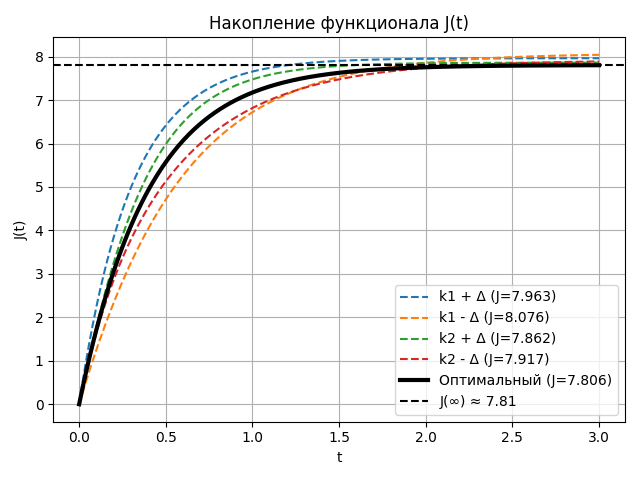
\includegraphics[width=0.8\textwidth]{images/J_comparison.png}
		\caption{Сравнительные графики накопления критериев качества}
		\label{fig:optim_j}
	\end{figure}
	\begin{figure}
		\centering
		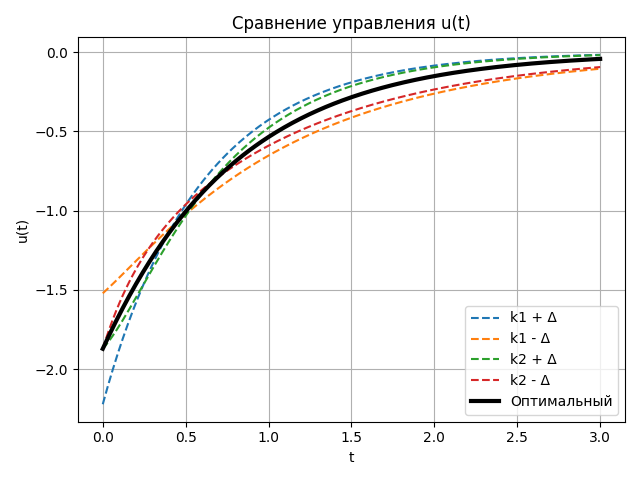
\includegraphics[width=0.8\textwidth]{images/u_comparison.png}
		\caption{Сравнительные графики управлений при отклонении $K$}
		\label{fig:u_comparison}
	\end{figure}
	\begin{figure}
		\centering
		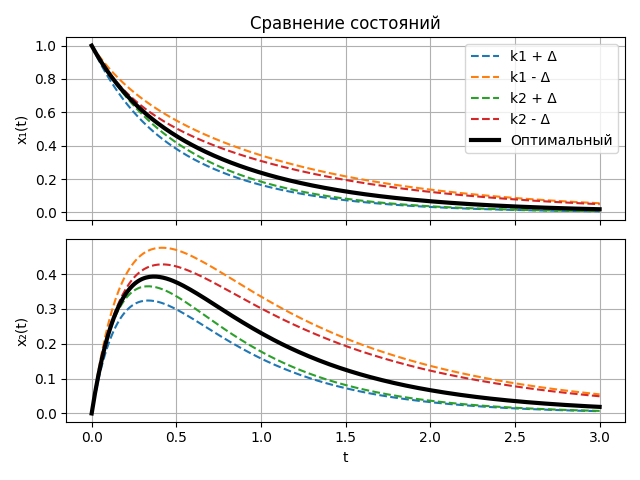
\includegraphics[width=0.8\textwidth]{images/x_comparison.png}
		\caption{Сравнительные графики состояний при отклонении $K$}
		\label{fig:x_comparison}
	\end{figure}

	Здесь стоит отметить, что отклонение коэффициентов обратной связи $K$ может приводить, например, к меньшим управлениям или более быстрой сходимости, что видно из сравнительных графиков управления (рисунок \ref{fig:u_comparison}) и состояний (рисунок \ref{fig:x_comparison}). Поэтому оптимальным регулятор является с точки зрения именно функционала с параметрами $Q \succcurlyeq 0$ и $r > 0$, задающих баланс между скоростью сходимости и величиной управления.

	\section{Общие выводы}
	В ходе лабораторной работы был синтезирован оптимальный регулятор для линейной системы с использованием метода динамического программирования Беллмана. Были рассчитаны коэффициенты обратной связи, которые минимизируют заданный функционал качества, и доказана оптимальность найденного решения путем сравнения с неоптимальными регуляторами. Моделирование подтвердило, что полученный закон управления успешно стабилизирует систему, приводя её состояния к нулю.
		

	


	
\end{document}